\section{Элементы защиты}
L и С выдержит пока не горит изоляция.
Основной элемент ПП - кристалл очень малых размеров

Трансформатор,реактор,мотор можно перегружать в десятки раз.
ПП -- граммы. Защита по току очень важна.

ПП -- прочность обратного pn-перехода ограничена. Малое время
для защиты по току(быстродействующая защита).
А по напряжению защит нет. Если перенапряжение состоялось, то всё
распространяется со скоростью света. Защита по напряжению, по недопущению
перенапряжения.

Из-за малой теплоемкости по току защита $10^{-3}...10^{-2}$. Существуют
быстродействующие плавкие предохранителию.

\begin{circuitikz}
  \draw (-0.2,1) node[left] {$I^2 t$ -- Мощность};
  \draw[->](0,0)--(0,2.2) node[left] {$I^2$};
  \draw[->](0,0)--(4,0) node[right] {$t$};
  \draw[domain=0.45:3.5]
  plot(\x, {1/\x});
\end{circuitikz}

Обычные плавкие предохранители олово+медь. Используется плавкая
вставка из технического серебра 99.9\% техническое чистое серебро
(драгоценный, но не благородный метал). Плавкая вставка должна быть
меньше чем ПП, чтобы быстро сгорела -- она должна быть горячей
в нормальном режиме.

$$
W = \left(\int I^2 dt\right)_\textcyrillic{тиристора} >
W_\textcyrillic{предохранителя}
$$
В этом случае тиристор может выдержать.

Все зависит от отношения
$$
\frac{I^2R}{c} \leftarrow \begin{array}{c}\textcyrillic{-- мощность}\\
  \textcyrillic{ -- теплоемкость}
 \end{array}
$$

\begin{circuitikz}
  \draw[->](0,0)--(0,3.2) node[left] {I};
  \draw[->](0,0)--(5.3,0) node[right] {t};
  \draw[domain=0:5]
  plot(\x,{-14*exp(-\x) + 14*exp(-0.6*\x)});
  \draw[domain=0:1]
  plot(\x,3.8*\x);
  \draw (0.7,0)--(0.7,2.2);
  \draw (1.8,0)--(1.8,2.4);
  \draw (3,0)--(3,1.6);
  \draw[<-] (2.2,2.5)--(3,2.8) node[right] {\begin{tabular}{l}
      расплавление\\
      дуга\\
      дуга растягивается
  \end{tabular}};
  \draw[<-] (0.7,-0.1)--(0,-0.4) node[left]
       {\begin{tabular}{l}время\\расплавления\end{tabular}};
  \draw (1.8,-0.4) node[below] {ограничение тока};
  \draw[<-] (3,-0.1)--(3.7,-0.4) node[right] {\begin{tabular}{l}время\\
       отключения\end{tabular}};    
\end{circuitikz}  

\section{Требования ключевого режима}
\begin{circuitikz}\draw
  (0,2)to[short,o-](1,2)--(1.5,2)--(2,2.4)
  (2,2)--(4,2)to[european resistor,l=$Z_\textcyrillic{н}$](4,0)to[short,-o](0,0)
  (1.8,2.4) node[above] {$V_K$}
  (1,2)--(1,2.9)
  (2.6,2)--(2.6,2.9)
  (0,1) node {$U_\textcyrillic{пит}$};
  \draw[->] (0.5,2.7)--(1,2.7);
  \draw[<-] (2.6,2.7)--(3.1,2.7) node[right] {$U_V$};
  \draw[<-] (1.75,1.8)--(1.75,1.3) node[right] {упр};
  \draw[->] (3.2,2.3)--(4,2.3)arc(90:0:0.4)--++(0,-0.1);
  \draw (6.9,1) node {\begin{tabular}{l}волна проводимости\\
      по сечению пробегает\\не мгновенно\end{tabular}}
  (11,1) node {\begin{tabular}{l}$V_D$\\$V_S$\\$V_T$\\
      $V_\textcyrillic{К}$ -- ключ по ГОСТ\end{tabular}}
;\end{circuitikz}  

\begin{circuitikz}
  \draw[->] (0,0)--(0,3.5) node[left] {};
  \draw[thin] (0,0)--(2.5,0) (3.5,0)--(6.5,0) (7,0)--(8.5,0);
  \draw[domain=0:2.5]
  plot (\x, {2.5*exp(-8*(\x-1)*(\x-1)*(\x-1)*(\x-1) -2*(\x-1)*(\x-1))+0.3});
  \draw[domain=3.5:6.5]
  plot (\x, {2.5*exp(-4*(\x-5)*(\x-5)*(\x-5)*(\x-5) -1*(\x-5)*(\x-5))+0.3});
  \draw[thin,snake=snake,segment amplitude = -0.4mm, segment length = 3mm] (2.5,0)--(2.5,2.7);
  \draw[thin,snake=snake,segment amplitude = 0.4mm, segment length = 3mm] (3.5,0)--(3.5,2.7);
  \draw[thin,snake=snake,segment amplitude = -0.4mm, segment length = 3mm] (6.5,0)--(6.5,2.7);
    \draw[thin,snake=snake,segment amplitude = 0.4mm, segment length = 3mm] (7,0)--(7,2.7);
  \draw[thin,loosely dashed] (0.3,3)--(0.3,0) node[below] {$t_1$};
  \draw[thin,loosely dashed] (1.7,3)--(1.7,0) node[below] {$t_2$};
  \draw[thin,<-] (0.3,3)--(0.1,3) node[midway,above] {u};
  \draw[thin] (0.3,3) -- (1.7,3) node[midway,above] {$\delta t_\textcyrillic{вкл}$};
  \draw[thin,<-] (1.7,3) -- (1.9,3);
  \draw[thin,loosely dashed] (4,3)--(4,0) node[below] {$t_3$};
  \draw[thin,loosely dashed] (6,3)--(6,0) node[below] {$t_4$};
  \draw[thin,loosely dashed] (7.3,3)--(7.3,0) node[below] {$t_5$};
  \draw[thin] (0.3,-0.5)--(0.3,-1.5) (6,-0.5)--(6,-1.5);
  \draw[thin,<->] (0.3,-1.3)--(6,-1.3) node[midway,above]
       {$T_K = \frac{1}{f_K}$};
  \draw[thin,<-] (4,3)--(3.8,3) node[midway,above] {};
  \draw[thin] (4,3) -- (6,3) node[midway,above] {$\delta t_\textcyrillic{выкл}$};
  \draw[thin,<-] (6,3) -- (6.2,3);
%  \draw[thin] (0,0)--(0,2.5) 
  \draw (4.2,2.3) node {$\scriptstyle{\Delta}p$};
  \draw [thin, <-] (4.3,2.2) -- (7.3,1) node[right] {\begin{tabular}{c}мгновенная\\
      мощность\end{tabular}};
  \draw (11.6,3) node {\begin{tabular}{c}как правило\\
      $\delta t_\textcyrillic{выкл} > t_\textcyrillic{вкл}$ \end{tabular}};
  \draw (11.6,1) node {\begin{tabular}{l}построим\\
      кривую мощности\\
      это тепло\\
  ${\scriptstyle \Delta}p = i_V U$\end{tabular}}
  ;\end{circuitikz}

Энергия в секунду $=$ мощность.

${\scriptstyle \Delta}P = \frac{w}{T_K}$ -- энергия в сек, мощность.

$=f_K \int\limits_{t_1}^{t_1 + T_K} U_V i_V dt $

где $f_K$ -- энергия потерь на переключении.

\begin{itemize}
\item мощность,выделяемая в открытом состоянии
  \item мощность в закрытом состоянии
\end{itemize}

$ 1) \gg 2) $

Чем больше частота, тем больше потери, но частоту нужно повышать.

\section{Основные типы полупроводниковых приборов}
Приборы неуправляемые -- диоды
\begin{circuitikz}
  \draw
  (0,1)to[D](0,0)
  (0,1)--(0,0)
  ;\end{circuitikz}

стабилитроны
\begin{circuitikz}
  \draw
  (0,0)to[D](0,1)
  (0,1)--(0,0)
  (0.18,0.62)--(0.18,0.5)
  ;\end{circuitikz}

КСОН -- кремниевый стабилизированный ограничитель напряжения.

варисторы
\begin{circuitikz}
  \draw
  (0,0)to[european resistor](1,0)
  (-0.1,-0.3)--(0.2,-0.3)--(0.8,0.3)
  ;\end{circuitikz}

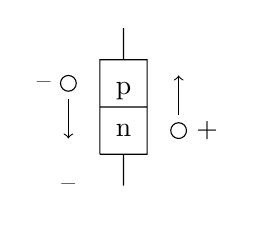
\begin{tikzpicture}\draw
  (0.4,0.4)--(1,0.4)--(1,1.6)--(0.4,1.6)--(0.4,0.4)
  (0.4,1)--(1,1)
  (0.7,0)--(0.7,0.4)
  (0.7,1.6)--(0.7,2)
  (0.7,0.7) node {n}
  (0.7,1.2) node {p}
  (1.4,0.7) circle(0.1) (1.5,0.7) node[right] {+}
  (0,1.3)circle(0.1) (-0.1,1.3) node[left] {--}
  (0,-0) node {--};
  \draw[->] (0,1.1) -- (0,0.6);
  \draw[->] (1.4,0.9) -- (1.4,1.4);
  
;\end{tikzpicture}

$$
\textcyrillic{транзисторы } 
\left\{\begin{tabular}{lcc}
МДП&--&метал-диэлектрик-полупроводник\\
МОП&--&метал-оксид-полупроводник\\
униполярные\\
с изолированным затвором\end{tabular}\right.
$$

\section{Вольт-амперная характеристика}
